% Editable source for the tree corresponding to kdt-1.tex.
% From this directory, regenerate with:
% latex -interaction=nonstopmode -halt-on-error kdt-2.tex
% dvisvgm --no-fonts --exact --bbox=papersize --output=kdt-2.svg kdt-2.dvi
\documentclass[tikz,border=5pt]{standalone}
\usepackage{lmodern}
\begin{document}
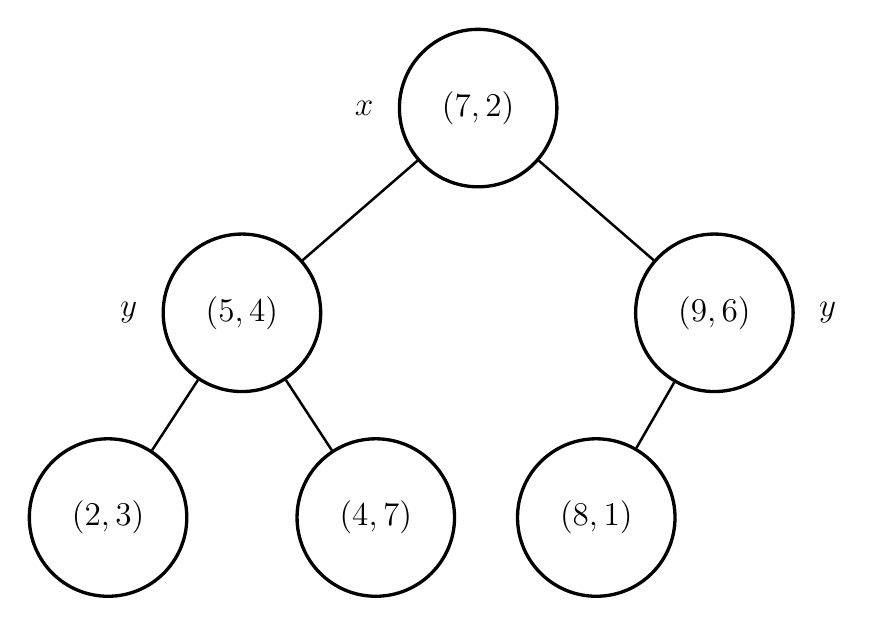
\begin{tikzpicture}[
  point/.style={circle,draw,line width=1.2pt,minimum size=20mm,inner sep=0pt},
  font=\large,line width=0.9pt
]
  % D is the root; C and E split the left and right regions along y.
  \node[point] (D) at (0,0) {$(7,2)$};
  \node[point] (C) at (-3,-2.6) {$(5,4)$};
  \node[point] (E) at (3,-2.6) {$(9,6)$};
  \node[point] (A) at (-4.7,-5.2) {$(2,3)$};
  \node[point] (B) at (-1.3,-5.2) {$(4,7)$};
  \node[point] (F) at (1.5,-5.2) {$(8,1)$};

  \draw (D) -- (C);
  \draw (D) -- (E);
  \draw (C) -- (A);
  \draw (C) -- (B);
  \draw (E) -- (F);

  \node[left=5pt] at (D.west) {$x$};
  \node[left=5pt] at (C.west) {$y$};
  \node[right=5pt] at (E.east) {$y$};
\end{tikzpicture}
\end{document}
